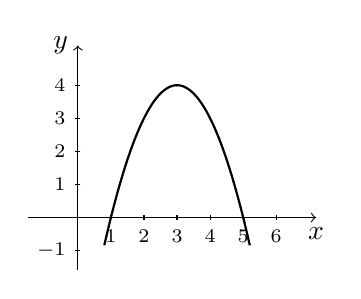
\begin{tikzpicture}[scale=0.42]
    \draw[->] (-1.5,0) -- (7.2,0) node[below] {$x$};
    \draw[->] (0,-1.6) -- (0,5.2) node[left] {$y$};
    \foreach \x in {1,2,3,4,5,6}
      \draw (\x,0.08)--(\x,-0.08) node[below] {\scriptsize $\x$};
    \foreach \y in {-1,1,2,3,4}
      \draw (0.08,\y)--(-0.08,\y) node[left] {\scriptsize $\y$};
    \draw[smooth, samples=200, domain=0.8:5.2, thick] plot (\x, {-(\x-3)*(\x-3)+4});
    \fill (1,0) circle (1.2pt);
    \fill (5,0) circle (1.2pt);
    \fill (3,4) circle (1.2pt);
\end{tikzpicture}
